\documentclass{article}
\usepackage{tikz}
\usepackage{tikz-3dplot}
\usepackage{ifthen}
\usetikzlibrary{calc}
\usepackage{amsmath}
\usepackage{amssymb}
\usetikzlibrary{arrows.meta, decorations.markings}

\tdplotsetmaincoords{70}{110}

\begin{document}

\def\glone{70}
\def\gltwo{70}
\def\glthree{-85}
\def\glfour{-60}
\def\glfive{70}
\def\glsix{70}

\def\gllone{0.5}
\def\glltwo{2}
\def\gllthree{1.5}
\def\gllfour{0.5}
\def\gllfive{1}
\def\gllsix{1}

\def\radius{1.1}    
\def\axlen{1.4}

\colorlet{Xcol}{red}
\colorlet{Ycol}{blue}
\colorlet{Zcol}{green}

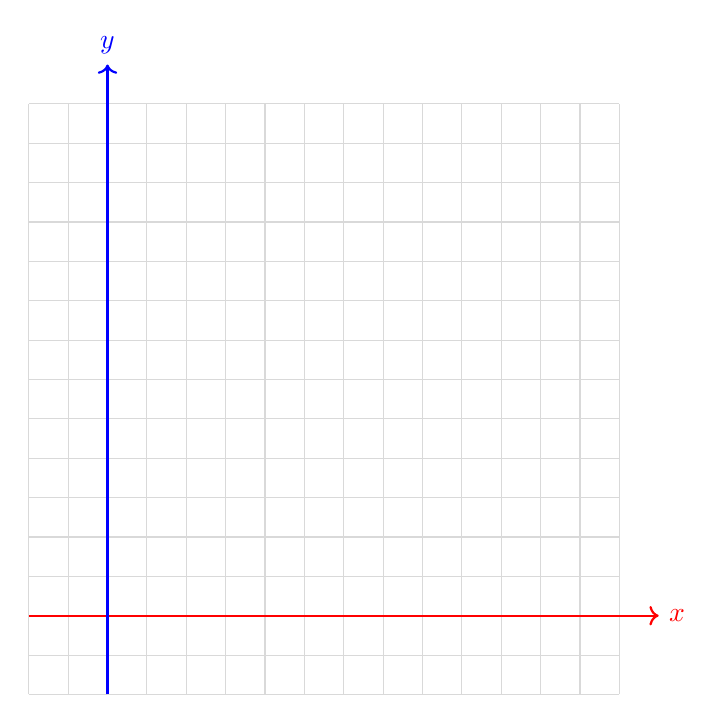
\begin{tikzpicture}[scale=2, thick]
  \draw[step=0.25, gray!30, thin] (-0.5, -0.5) grid (3.25, 3.25);
  \draw[->, red] (-0.5,0) -- (3.5,0) node[right] {$x$};
  \draw[->, blue] (0,-0.5) -- (0,3.5) node[above] {$y$};
\end{tikzpicture}

\begin{tikzpicture}[scale=2, thick]
  \draw[step=0.25, gray!30, thin] (-0.5, -0.5) grid (3.25, 3.25);
  \draw[->, gray!70] (-0.5,0) -- (3.5,0) node[right] {$x$};
  \draw[->, gray!70] (0,-0.5) -- (0,3.5) node[above] {$y$};

  \coordinate (O) at (0, 0);
  \coordinate (A) at ({\glltwo * cos(\gltwo)}, {\glltwo * sin(\gltwo)});
  
  \draw[thin, dashed] plot[domain=-14.5:104.5, samples=180] ({\glltwo*cos(\x)},{\glltwo*sin(\x)});

  %\draw[->, thin, thick, orange] plot[domain=0:\gltwo, samples=180] ({0.4*cos(\x)},{0.4*sin(\x)});
  %\node[below left, orange] at ({0.39*cos(\gltwo/2)},{0.47*sin(\gltwo/2)}) {$\theta$};

  \draw[-, orange, ultra thick, line cap=round] (O) -- (A) node[pos=0.5, above left] {$L_1$};
\end{tikzpicture}

\begin{tikzpicture}[scale=2, thick]
  \draw[step=0.25, gray!30, thin] (-0.5, -0.5) grid (3.25, 3.25);
  \draw[->, gray!70] (-0.5,0) -- (3.5,0) node[right] {$x$};
  \draw[->, gray!70] (0,-0.5) -- (0,3.5) node[above] {$y$};

  \coordinate (O) at (0, 0);
  \coordinate (A) at ({\glltwo * cos(\gltwo)}, {\glltwo * sin(\gltwo)});
  \path (A) +({\gllthree * cos(\glthree + \gltwo)}, {\gllthree * sin(\glthree + \gltwo)}) coordinate (B);

  %\draw[dashed, black, semithick] (A) ++(0, 0) -- ++({0.4 * cos(\gltwo)}, {0.4* sin(\gltwo)});
  %\draw[->, thick, orange] plot[domain=\gltwo :{\glthree + \gltwo}, samples=180] ({\glltwo * cos(\gltwo) + 0.4*cos(\x)},{\glltwo * sin(\gltwo) + 0.4*sin(\x)});
  %\node[below left, orange] at ({\glltwo * cos(\gltwo) + 0.36*cos(\gltwo + \glthree/2)},{\glltwo * sin(\gltwo) + 0.50*sin(\gltwo + \glthree/2)}) {$\theta$};
  
  \draw[-, black, very thick, line cap=round] (O) -- (A) node[pos=0.5, above left] {$L_1$};
  \draw[-, orange, very thick, line cap=round] (A) -- (B) node[pos=0.5, above] {$L_2$};

  \draw[<->, red]  (B)++(-0.2, 0)-- (B) -- ++(0.2, 0);
  \draw[<->, blue]  (B)++(0, -0.2)-- (B) -- ++(0, 0.2);
\end{tikzpicture}

\begin{tikzpicture}[scale=2, thick]
  \draw[step=0.25, gray!30, thin] (-0.5, -0.5) grid (3.25, 3.25);
  \draw[->, gray!70] (-0.5,0) -- (3.5,0) node[right] {$x$};
  \draw[->, gray!70] (0,-0.5) -- (0,3.5) node[above] {$y$};

  \coordinate (O) at (0, 0);
  \coordinate (A) at ({\glltwo * cos(\gltwo)}, {\glltwo * sin(\gltwo)});
  \path (A) +({\gllthree * cos(\glthree + \gltwo)}, {\gllthree * sin(\glthree + \gltwo)}) coordinate (B);
  \path (B) +({\gllfour * cos(\glfour + \glthree + \gltwo)}, {\gllfour * sin(\glfour + \glthree + \gltwo)}) coordinate (C);
  
  \draw[-, black, very thick, line cap=round] (O) -- (A) node[pos=0.5, above left] {$L_1$};
  \draw[-, black, very thick, line cap=round] (A) -- (B) node[pos=0.5, above] {$L_2$};
  \draw[-, orange, very thick, line cap=round] (B) -- (C) node[pos=0.5, right] {$L_3$};

  \draw[<->, red]  (C)++(-0.2, 0)-- (C) -- ++(0.2, 0);
  \draw[<->, blue]  (C)++(0, -0.2)-- (C) -- ++(0, 0.2);
  \draw[->, green] plot[domain=-180:-90, samples=180] ({\gllfour * cos(\glfour + \glthree + \gltwo) + \gllthree * cos(\glthree + \gltwo) + \glltwo * cos(\gltwo) + 0.3*cos(\x)}, {\gllfour * sin(\glfour + \glthree + \gltwo) + \gllthree * sin(\glthree + \gltwo) + \glltwo * sin(\gltwo) + 0.3*sin(\x)});
\end{tikzpicture}



% ---------- Rotation about Z (in the XY-plane) ----------
\begin{tikzpicture}[tdplot_main_coords, scale=2]
  % axes
  \draw[->] (0,0,0) -- (\axlen,0,0) node[below left] {\textcolor{Xcol}{$x$}};
  \draw[->] (0,0,0) -- (0,\axlen,0) node[right]  {\textcolor{Ycol}{$y$}};
  \draw[->] (0,0,0) -- (0,0,\axlen) node[above]  {\textcolor{Zcol}{$z$}};

  % circle in XY-plane
  \draw[thin, dashed] (0,0,0) ++(\radius,0,0) arc (0:360:\radius);

  % original x-axis point
  \coordinate (X0) at (\radius,0,0);
  % rotated point (by alpha around z) (cos, sin, 0)
  \coordinate (Xr) at ({\radius*cos(45)},{\radius*sin(45)},0);

  % arc showing rotation
  \draw[->, thick, Zcol] plot[domain=0:45, samples=50] ({\radius*cos(\x)},{\radius*sin(\x)},0);

  % vectors
  \draw[-, thick, Zcol] (0,0,0) -- (Xr) node[pos=1.3, below] {$\mathbf{R}_z(\psi)$};

  % angle label
  \node at ({0.55*\radius*cos(22.5)},{0.2*\radius*sin(22.5)},0) [right] {$\psi$};
\end{tikzpicture}
\vspace{20mm}
\hspace{40mm}

% ---------- Rotation about X (in the YZ-plane) ----------
\begin{tikzpicture}[tdplot_main_coords, scale=2]
  % axes
  \draw[->] (0,0,0) -- (\axlen,0,0) node[below left] {\textcolor{Xcol}{$x$}};
  \draw[->] (0,0,0) -- (0,\axlen,0) node[right]  {\textcolor{Ycol}{$y$}};
  \draw[->] (0,0,0) -- (0,0,\axlen) node[above]        {\textcolor{Zcol}{$z$}};

  % circle in YZ-plane (centered at origin, param: (0, cos t, sin t))
  \draw[thin, dashed] plot[domain=0:360, samples=180] (0,{\radius*cos(\x)},{\radius*sin(\x)});

  % original y-axis point
  \coordinate (Y0) at (0,\radius,0);
  % rotated point (by beta about x): (0, cos(beta), sin(beta))
  \coordinate (Yr) at (0,{\radius*cos(45)},{\radius*sin(45)});

  % arc showing rotation
  \draw[->, thick, Xcol] plot[domain=0:45, samples=50] (0,{\radius*cos(\x)},{\radius*sin(\x)});

  % vectors
  \draw[-, thick, Xcol] (0,0,0) -- (Yr) node[pos=1.1, right ] {$\mathbf{R}_x(\varphi)$};

  % angle label
  \node at (0,{0.7*\radius*cos(22.5)},{0.6*\radius*sin(22.5)}) [left] {$\varphi$};

\end{tikzpicture}
\vspace{20mm}
\hspace{40mm}


% ---------- Rotation about Y (in the XZ-plane) ----------
\begin{tikzpicture}[tdplot_main_coords, scale=2]
  % axes
  \draw[->] (0,0,0) -- (\axlen,0,0) node[below left] {\textcolor{Xcol}{$x$}};
  \draw[->] (0,0,0) -- (0,\axlen,0) node[right]  {\textcolor{Ycol}{$y$}};
  \draw[->] (0,0,0) -- (0,0,\axlen) node[above]        {\textcolor{Zcol}{$z$}};

  % circle in XZ-plane (param: (cos t, 0, sin t))
  \draw[thin, dashed] plot[domain=0:360, samples=180] ({\radius*cos(\x)},0,{\radius*sin(\x)});

  % original x-axis point
  \coordinate (X0b) at (\radius,0,0);
  % rotated point (by gamma about y): (cos gamma, 0, sin gamma)
  \coordinate (Xrb) at ({\radius*cos(45)},0,{\radius*sin(45)});

  % arc showing rotation
  \draw[->, thick, Ycol] plot[domain=0:45, samples=50] ({\radius*cos(\x)},0,{\radius*sin(\x)});

  \draw[-, thick, Ycol] (0,0,0) -- (Xrb) node[pos=0.95, above left] {$\mathbf{R}_y(\theta)$};

  % angle label
  \node at ({0.6*\radius*cos(22.5)},0,{0.8*\radius*sin(22.5)}) [below] {$\gamma$};
\end{tikzpicture}

% Forward Kinematics with objective angles
\begin{tikzpicture}[scale=2, thick]

  
  \def\lone{2.0}
  \def\ltwo{2.0}

  
  \def\thetaone{35}   % theta1
  \def\thetatwo{40}   % theta2 (relative!)

  % Coordinates of joint 1 (origin)
  \coordinate (O) at (0,0);

  % End of first link
  \coordinate (A) at ({\lone*cos(\thetaone)}, {\lone*sin(\thetaone)});

  % End of second link (theta1+theta2)
  \coordinate (B) at ({\lone*cos(\thetaone) + \ltwo*cos(\thetaone+\thetatwo)},
                      {\lone*sin(\thetaone) + \ltwo*sin(\thetaone+\thetatwo)});

  % Draw base axes
  \draw[->, gray!70] (-0.5,0) -- (3.5,0) node[right] {$x$};
  \draw[->, gray!70] (0,-0.5) -- (0,3.5) node[above] {$y$};

  \filldraw[black] (O) circle (1.2pt);
  \filldraw[black] (A) circle (1.2pt);
  \filldraw[black] (B) circle (1.2pt) node[above] {$X_\mathbf{D}$};
  
  % Draw links
  \draw[very thick] (O) -- (A) node[midway, above left] {$l_1$};
  \draw[very thick] (A) -- (B) node[midway, above left] {$l_2$};
  


  

  \filldraw[black] (O) circle (0.35pt);
  \filldraw[black] (A) circle (0.35pt);

  % Angle theta1 at origin
  \draw[->] (0.8,0) arc[start angle=0, end angle=\thetaone, radius=0.8];
  \node at (0.9,0.3) {$\theta_1$};

  % Angle theta2 at joint A (relative!)
  \draw[->] (A) ++(0.8,0) arc[start angle=0, end angle=\thetaone+\thetatwo, radius=0.8];
  \draw[-, dashed] (A)++(0.8, 0) -- (A);
  \node at ({1.3*cos(\thetaone+0.5*\thetatwo) + \lone*cos(\thetaone)}, {0.8*sin(\thetaone+0.5*\thetatwo) + \lone*sin(\thetaone)}) {$\theta_2$};

  \draw[->, ultra thick, red, line cap=rect] (O) -- (0.5, 0);
  \draw[->, ultra thick, blue, line cap=rect] (O) -- (0, 0.5);

  \draw[->, ultra thick, red, line cap=rect]  (A) -- ++(0.5, 0);
  \draw[->, ultra thick, blue, line cap=rect]  (A) --  ++(0, 0.5);
\end{tikzpicture}

% Forward Kinematics with relative angles
\begin{tikzpicture}[scale=2, thick]

  
  \def\lone{2.0}
  \def\ltwo{2.0}

  
  \def\thetaone{35}   % theta1
  \def\thetatwo{40}   % theta2 (relative!)

  % Coordinates of joint 1 (origin)
  \coordinate (O) at (0,0);

  % End of first link
  \coordinate (A) at ({\lone*cos(\thetaone)}, {\lone*sin(\thetaone)});

  % End of second link (theta1+theta2)
  \coordinate (B) at ({\lone*cos(\thetaone) + \ltwo*cos(\thetaone+\thetatwo)},
                      {\lone*sin(\thetaone) + \ltwo*sin(\thetaone+\thetatwo)});

  % Draw base axes
  \draw[->, gray!70] (-0.5,0) -- (3.5,0) node[right] {$x$};
  \draw[->, gray!70] (0,-0.5) -- (0,3.5) node[above] {$y$};

  \filldraw[black] (O) circle (1.2pt);
  \filldraw[black] (A) circle (1.2pt);
  \filldraw[black] (B) circle (1.2pt) node[above] {$X_\mathbf{D}$};
  
  % Draw links
  \draw[very thick] (O) -- (A) node[midway, above left] {$l_1$};
  \draw[very thick] (A) -- (B) node[midway, above left] {$l_2$};
  


  \draw[->, ultra thick, red, line cap=rect] (O) -- ({0.5*cos(\thetaone)},{0.5*sin(\thetaone)});
  \draw[->, ultra thick, blue, line cap=rect] (O) -- ({0.5*cos(\thetaone + 90)},{0.5*sin(\thetaone + 90)});

  \draw[->, ultra thick, red, line cap=rect]  (A) -- ++({0.5*cos(\thetaone + \thetatwo)},{0.5*sin(\thetaone + \thetatwo)});
  \draw[->, ultra thick, blue, line cap=rect]  (A) --  ++({0.5*cos(\thetaone + \thetatwo + 90)},{0.5*sin(\thetaone + \thetatwo + 90)});

  \filldraw[black] (O) circle (0.35pt);
  \filldraw[black] (A) circle (0.35pt);

  % Angle theta1 at origin
  \draw[->] (0.8,0) arc[start angle=0, end angle=\thetaone, radius=0.8];
  \node at (0.9,0.3) {$\theta_1$};

  % Angle theta2 at joint A (relative!)
  \draw[->] (A) ++({0.8*cos(\thetaone)},{0.8*sin(\thetaone)}) arc[start angle=\thetaone, end angle=\thetaone+\thetatwo, radius=0.8];
  \draw[-, dashed] (A)++({0.8*cos(\thetaone)},{0.8*sin(\thetaone)}) -- (A);
  \node at ({1*cos(\thetaone+0.5*\thetatwo) + \lone*cos(\thetaone)}, {1*sin(\thetaone+0.5*\thetatwo) + \lone*sin(\thetaone)}) {$\theta_2$};


\end{tikzpicture}

\end{document}